\section{Exploding Gradients (Patlayan Gradyanlar Problemi)}
Eğitim sırasında, gradyanlar belirli bir eşiğin üzerine çıkar ve bu da ağın aşırı derecede büyük güncellemeler yapmasına neden olabilir. 

\begin{figure}[h]
    \centering
    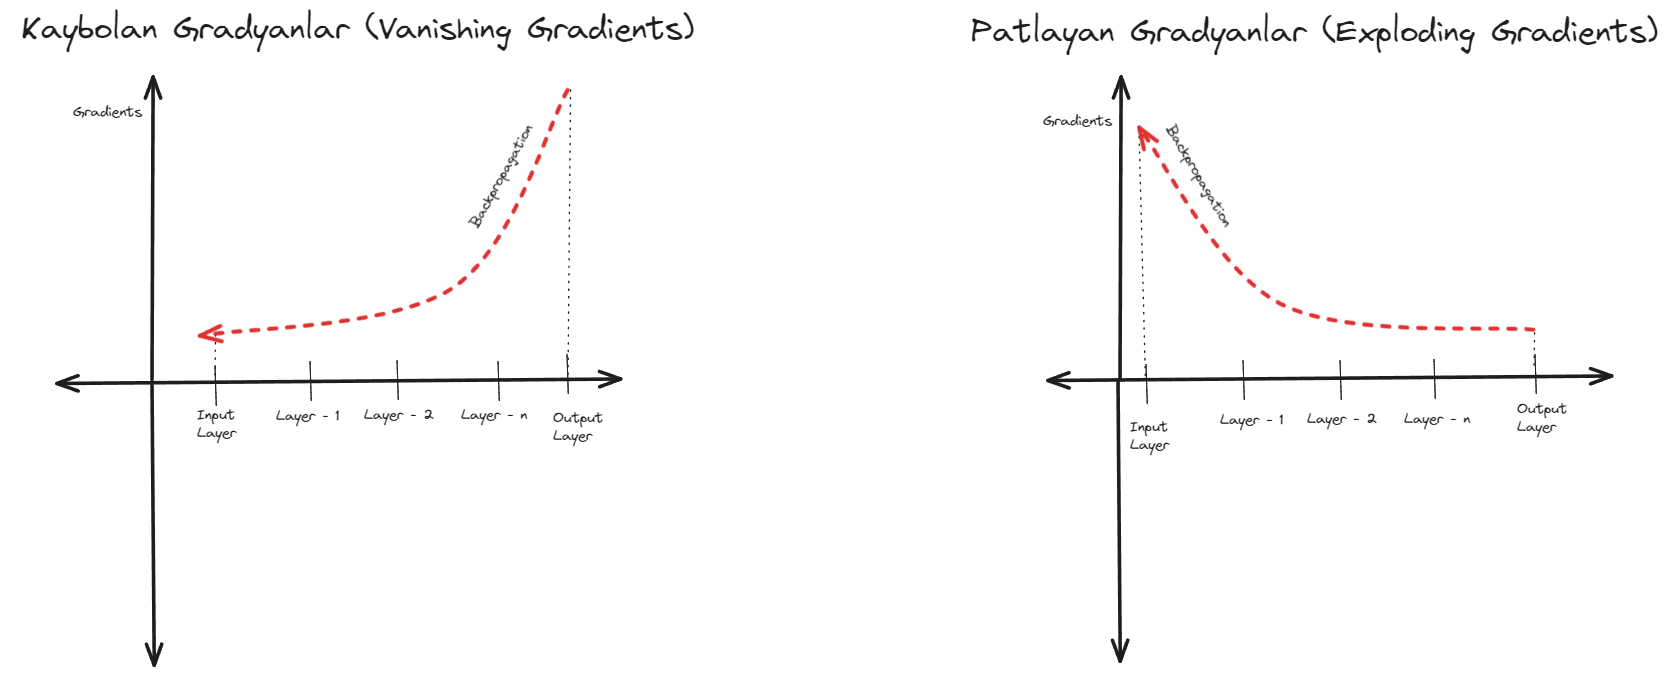
\includegraphics[width=1\textwidth]{images/gradient_problems.png}
    \caption{Gradyan problemleri.}
    \label{fig:enter-label}
\end{figure}

\subsubsection{Ortaya Çıkışı}
\begin{itemize}
    \item Ağın öğrenme oranı çok yüksekse, gradyanlar hızla büyüyebilir ve kontrol edilemeyen güncellemelere neden olabilir.
    \item Derin sinir ağları genellikle birçok katmandan oluşur ve bu katmanlar arasında geriye doğru gradyanlar aktarılır. Bu süreçte, gradyanlar katmanlardan katmanlara geçerken büyüyebilir ve patlayabilir.
\end{itemize}

\subsubsection{Engelleme Yöntemleri}
\begin{itemize}
    \item Gradyanları belirli bir eşiğin altında veya üstünde tutmak için kısıtlama işlemi uygulanabilir. Bu, gradyanların patlamasını önler ve modelin daha istikrarlı bir şekilde eğitilmesini sağlar.
    \item Öğrenme oranı, gradyanların büyümesini kontrol etmek için düşürülebilir. Daha düşük bir öğrenme oranı, daha yavaş ve istikrarlı bir eğitim süreci sağlar.
\end{itemize}

\newpage